\begin{frame}{Performance in Controllable Protein Generation}% on Four Different Instructions
	\begin{center}
		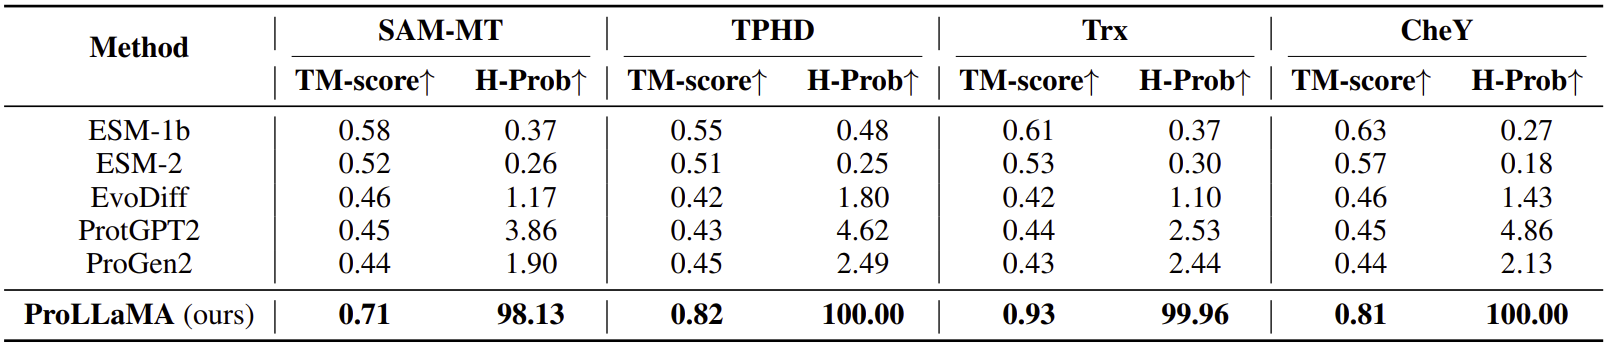
\includegraphics[scale=0.21]{tables/controlled_generation_comparison.png}
	\end{center}
	\vspace{-1em}\credit{Table}{lv2024prollama}
	\begin{itemize}
		\item Given one instruction, \\ProLLaMA generates proteins with the desired functionalities
		\item High metrics mean proteins meet instructions
		\item Other models: uncontrollable generation
		\item Instructions: four superfamily descriptions
		%What do superfamilies are?
		\begin{itemize}
			\item SAM-MT: S-adenosyl-L-methionine-dependent methyltransferase
			\item TPHD: Tetratricopeptide-like helical domain
			\item Trx: Thioredoxin-like 
			\item CheY: CheY-like
		\end{itemize}
	\end{itemize}
\end{frame}